\documentclass[conference]{IEEEtran}
\usepackage{iftex}
\ifPDFTeX
  \usepackage[T1]{fontenc}
\else  % XeLaTeX / Tectonic: Times-compatible OpenType font
  \usepackage{fontspec}
  \setmainfont{texgyretermes}[Extension=.otf, UprightFont=*-regular, BoldFont=*-bold,
    ItalicFont=*-italic, BoldItalicFont=*-bolditalic]
\fi
\usepackage{amsmath,amssymb,amsfonts}
\usepackage{graphicx}
\usepackage{booktabs}
\usepackage{multirow}
\usepackage{xcolor}
\usepackage{url}
\usepackage[hidelinks]{hyperref}
\usepackage{cite}
\graphicspath{{../results/figures/}}

\newcommand{\R}{\mathbb{R}}
\newcommand{\vect}[1]{\mathbf{#1}}

\begin{document}

\title{Spatio-Temporal Traffic Speed Forecasting on METR-LA:\\
From Engineered Features to Graph Neural Networks}

% TODO: replace the placeholders below with your details.
\author{\IEEEauthorblockN{Student Name 1, Student Name 2}
\IEEEauthorblockA{\textit{Department of Computer Science, Institution Name}\\
City, Country\\
email@institution.edu}
}

\maketitle

\begin{abstract}
Placeholder abstract.

\end{abstract}

\begin{IEEEkeywords}
traffic forecasting, spatio-temporal data, graph neural networks, Graph WaveNet,
gradient boosting, feature engineering, METR-LA
\end{IEEEkeywords}

\section{Introduction}
Accurate short-term traffic forecasts underpin route guidance, ramp metering,
incident response and travel-time estimation in Intelligent Transportation
Systems~\cite{vlahogianni2014}. Forecasting freeway speed is hard for four
reasons that are all visible in real sensor data: the dynamics are strongly
\emph{non-linear} near the onset of congestion; the series are
\emph{seasonal} (daily and weekly demand cycles); congestion
\emph{propagates spatially} along the road network; and loop detectors
frequently \emph{fail}, producing missing readings.

Research has moved from univariate statistical models (ARIMA~\cite{ahmed1979,williams2003})
through feature-based machine learning~\cite{smith1997} and recurrent networks~\cite{ma2015lstm}
to spatio-temporal graph neural networks (GNNs) that treat the sensor network as a
graph~\cite{li2018dcrnn,yu2018stgcn,wu2019gwnet}. Published comparisons, however,
often pit sophisticated GNNs against feature-poor classical baselines, and rarely
test whether accuracy differences are statistically significant.

This paper studies 1-hour-ahead speed forecasting on the METR-LA
benchmark~\cite{li2018dcrnn} and makes the following contributions:
\begin{enumerate}
\item A data-quality and exploratory analysis that quantifies missingness,
seasonality, stationarity and spatial dependence. It links each finding to a
modelling decision.
\item A leakage-tested feature set (34 features in six groups) that includes a weekly
profile/anomaly decomposition and upstream/downstream graph aggregates. Its value
is measured by cumulative ablation and permutation importance.
\item A controlled ladder of six forecasters (Historical Average, Persistence,
Ridge, gradient boosting, LSTM and Graph WaveNet~\cite{wu2019gwnet}) evaluated
under the standard protocol. We compare against published results and report
Diebold--Mariano tests~\cite{diebold1995} and block-bootstrap confidence intervals.
\item An ablation of Graph WaveNet's spatial module (none, road graph, adaptive
graph, both) under an equal budget, plus error analyses by horizon, time of day,
sensor and missing input.
\end{enumerate}
All code, tests and results are released in the project repository.

\section{Related Work}
\textbf{Statistical models.} Ahmed and Cook~\cite{ahmed1979} first applied
Box--Jenkins ARIMA to freeway data, and Williams and Hoel~\cite{williams2003}
justified seasonal ARIMA by showing that weekly-differenced traffic is
stationary. These models are univariate and linear, and they degrade quickly with
horizon: on METR-LA, ARIMA's MAE rises from 3.99 to 6.90\,mph between 15 and
60\,min~\cite{li2018dcrnn}.

\textbf{Feature-based machine learning.} Non-parametric regression (k-NN) was shown
to be competitive and robust~\cite{smith1997}. Tree ensembles~\cite{breiman2001}
and gradient boosting~\cite{friedman2001,ke2017lightgbm} model non-linear
interactions but depend heavily on feature engineering. In the DCRNN benchmark,
SVR on raw lags reached only 6.72\,mph at 60\,min~\cite{li2018dcrnn}.

\textbf{Deep sequence models.} Stacked autoencoders~\cite{lv2015} and
LSTMs~\cite{hochreiter1997,ma2015lstm} learn temporal representations directly.
Encoder--decoder (FC-)LSTMs~\cite{sutskever2014} predict a whole horizon and reach
4.37\,mph at 60\,min on METR-LA~\cite{li2018dcrnn}, but they ignore road topology.

\textbf{Spatio-temporal GNNs.} Spectral~\cite{defferrard2016} and
first-order~\cite{kipf2017} graph convolutions made it possible to exploit
topology. DCRNN~\cite{li2018dcrnn} models traffic as a bidirectional diffusion
process on a directed distance graph inside a GRU seq2seq. STGCN~\cite{yu2018stgcn}
replaces recurrence with gated temporal convolutions, and ASTGCN~\cite{guo2019astgcn}
adds attention. Graph WaveNet~\cite{wu2019gwnet} combines diffusion convolution
with dilated causal convolutions~\cite{oord2016wavenet} and a \emph{self-adaptive}
adjacency learned from node embeddings, showing that the predefined graph is
incomplete. Later work learns the graph entirely (MTGNN~\cite{wu2020mtgnn},
AGCRN~\cite{bai2020agcrn}), uses attention (GMAN~\cite{zheng2020gman},
STAEformer~\cite{liu2023staeformer}), or shows that simple spatial and temporal
identity embeddings recover much of the gain (STID~\cite{shao2022stid}).
Jiang and Luo~\cite{jiang2022survey} survey the area.

\textbf{Positioning.} We adopt Graph WaveNet as our representative GNN. It is
accurate, convolutional (so it trains on modest hardware) and lets us ablate both
the predefined and the learned graph. We pair it with strong, leakage-free feature
baselines and add significance testing, which the literature rarely reports.

\section{Dataset and Exploratory Analysis}
\label{sec:data}

\subsection{METR-LA}
METR-LA~\cite{jagadish2014,li2018dcrnn} contains 5-minute average speeds from
$N{=}207$ loop detectors on Los Angeles County freeways, from 1~March to 27~June
2012 ($T{=}34{,}272$ steps; Table~\ref{tab:data}). It ships with sensor
coordinates and 295,374 directed road-network distances, of which 11,753 are
between sensors in the dataset. The HDF5 file was written by pandas~0.15, so we
read its arrays directly with \texttt{h5py}.

\begin{table}[t]
\centering
\caption{Dataset summary (computed by \texttt{scripts/run\_eda.py}).}
\label{tab:data}
\begin{tabular}{ll}
\toprule
Sensors / time steps & 207 / 34,272 (119 days, 5 min) \\
Missing readings (value $=0$) & 8.11\,\% (per sensor 6.3--20.1\,\%) \\
Observed speed mean $\pm$ std & 58.5 $\pm$ 13.0 mph (median 63.2) \\
Readings $<$ 40 mph (congested) & 10.9\,\% \\
Skewness & $-1.99$ \\
Graph non-zeros (incl.\ self-loops) & 1,722 (1,515 directed edges) \\
One-way edges & 73.3\,\% \\
Split (windows) & 23,974 / 3,425 / 6,850 \\
\bottomrule
\end{tabular}
\end{table}

\subsection{Data quality}
Missing observations are encoded as $0$\,mph, which is physically implausible on a
freeway. They make up 8.1\,\% of readings. Fig.~\ref{fig:missing} shows two
mechanisms: network-wide outages (vertical stripes, e.g.\ 26--27~March, when
$>$50\,\% of readings are missing) and long single-sensor failures (the median
sensor's longest gap is 381 steps, about 32\,h). Speeds are capped at 70\,mph by the
sensors' processing. We therefore (i) mask zero targets out of every loss and metric,
(ii) never impute labels, and (iii) use only \emph{causal} forward-filling (last
observation carried forward) when building features. Interpolation would use future
values.

\begin{figure*}[t]
\centering
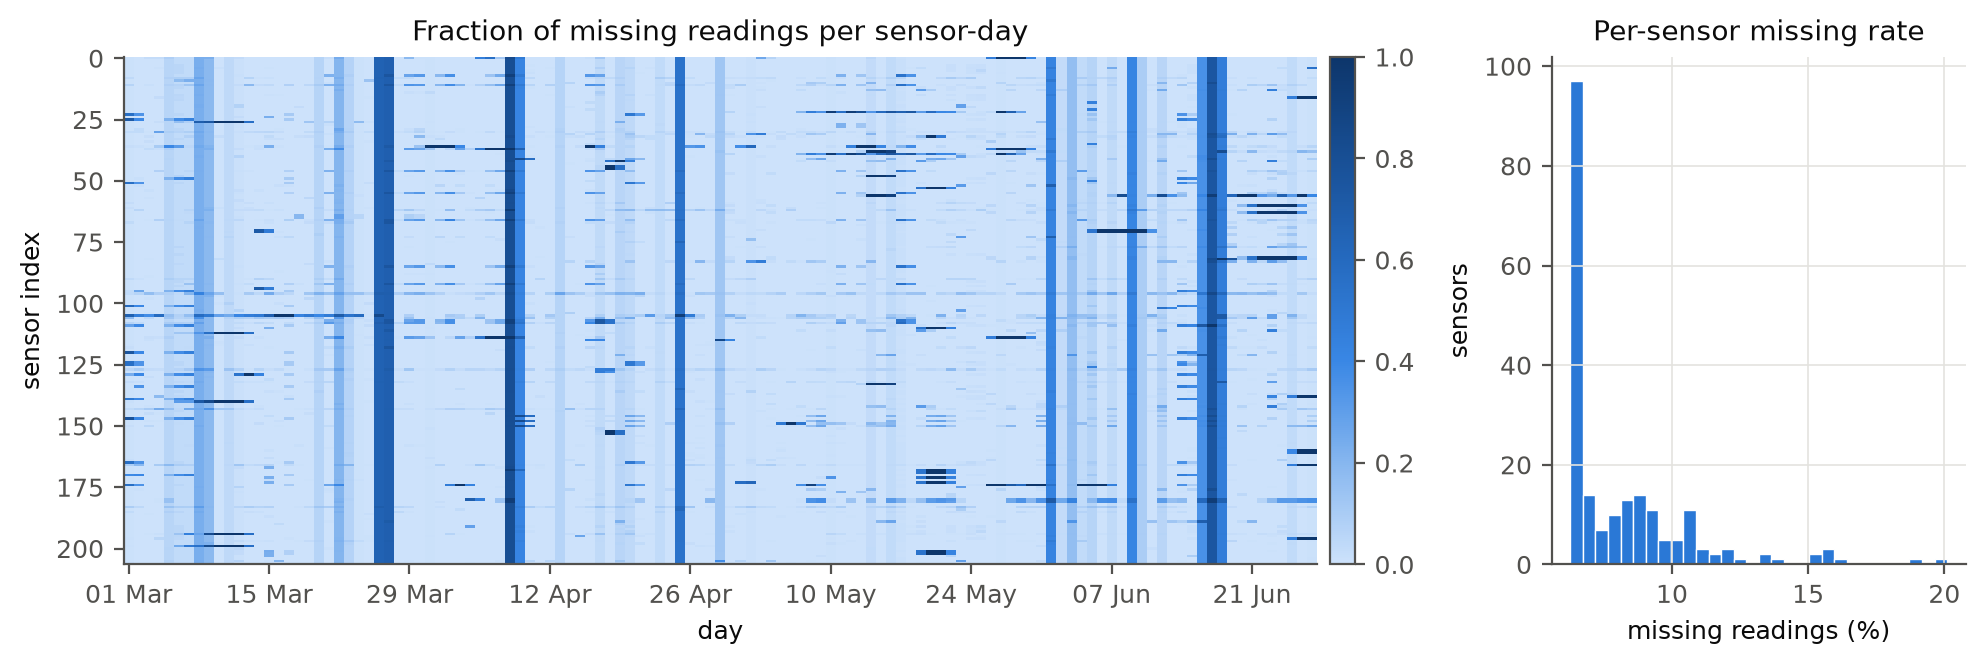
\includegraphics[width=0.85\textwidth]{eda_missingness.png}
\caption{Missingness. Left: fraction of zero readings per sensor-day. Vertical
stripes are network outages; horizontal streaks are sensor failures. Right:
distribution of per-sensor missing rates.}
\label{fig:missing}
\end{figure*}

\subsection{Temporal structure}
Weekday speeds show a pronounced evening rush hour (network mean 45.2\,mph at
17:30) and a weaker morning dip, while weekends are flat (minimum 56.8\,mph;
Fig.~\ref{fig:profile}). The autocorrelation function (Fig.~\ref{fig:acf}) is
0.86 at lag 5\,min and 0.57 at 1\,h. It peaks every 24\,h, with the 168\,h peak
(0.40) above the 24\,h peak (0.36), so the seasonality is weekly. Subtracting each
sensor's weekly profile (fitted on training data) removes the daily peaks: the
24\,h ACF falls from 0.36 to 0.07. The residual \emph{anomaly} is a short-memory
process (ACF 0.41 at 1\,h). This additive decomposition, speed = weekly profile +
anomaly, motivates several features. Augmented Dickey--Fuller
tests~\cite{dickey1979} reject a unit root for all ten sampled sensors
($p<10^{-24}$), so the series need no differencing; their non-stationarity is
seasonal, not a stochastic trend.

\begin{figure*}[t]
\centering
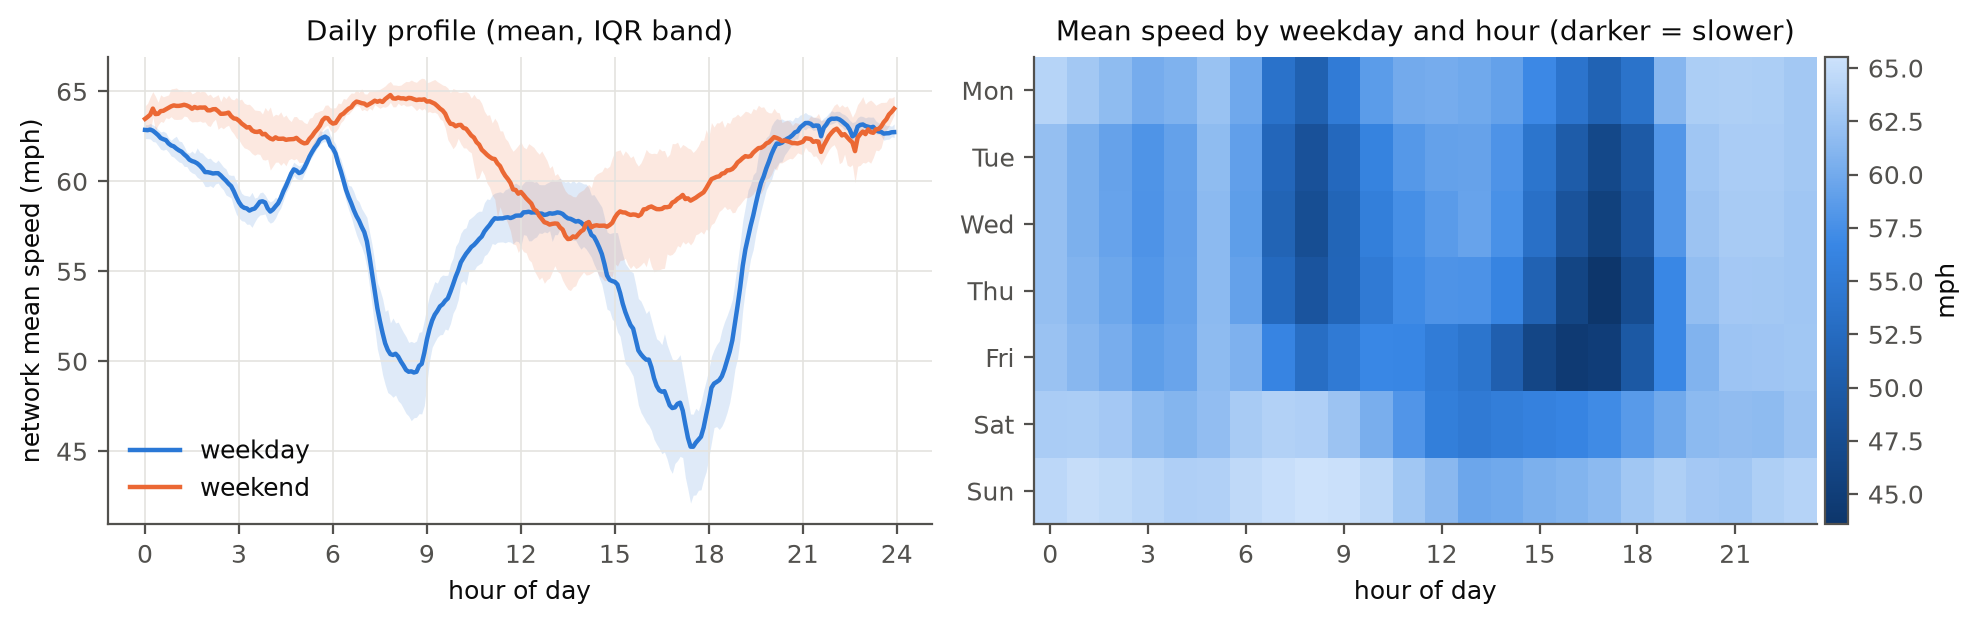
\includegraphics[width=0.9\textwidth]{eda_daily_profile.png}
\caption{Left: network-mean speed by time of day (line: mean; band: inter-quartile
range across days). Right: mean speed by weekday and hour.}
\label{fig:profile}
\end{figure*}

\begin{figure}[t]
\centering
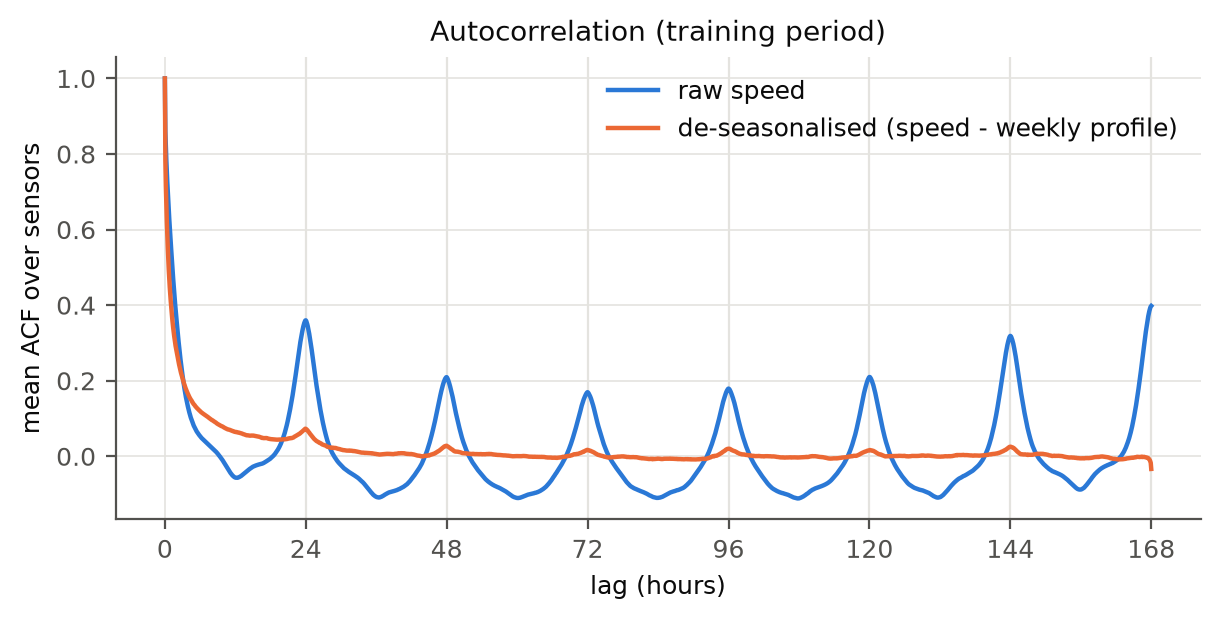
\includegraphics[width=\columnwidth]{eda_acf.png}
\caption{Mean autocorrelation over sensors, for raw speeds and after removing the
weekly profile.}
\label{fig:acf}
\end{figure}

\subsection{Spatial structure}
Pairwise correlation decays with road distance (Fig.~\ref{fig:spatial}), and the
decay persists after de-seasonalising, so it is not just a shared daily cycle.
Graph-connected sensors have a mean anomaly correlation of 0.27, against 0.07 for
pairs with no recorded road path. The Spearman correlation between distance and
anomaly correlation is $-0.20$. The distance graph is strongly directed: 73\,\%
of edges have no reverse edge, and five sensors have no outgoing edge. This
justifies both direction-aware spatial features and a learned adjacency.

\begin{figure}[t]
\centering
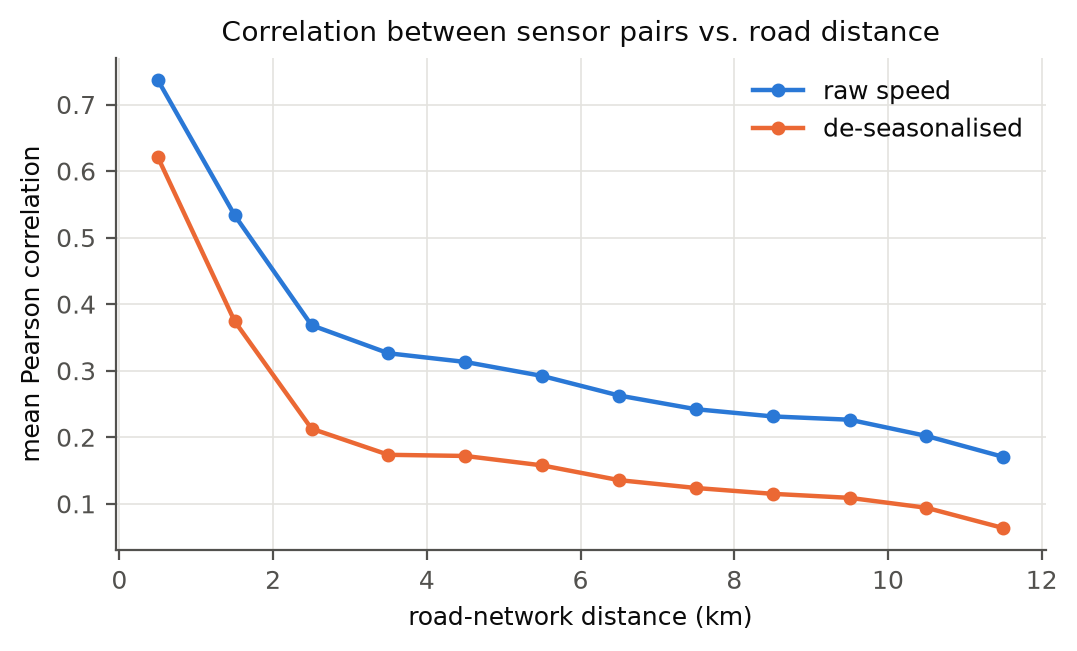
\includegraphics[width=\columnwidth]{eda_spatial_corr.png}
\caption{Mean Pearson correlation between sensor pairs, binned by road distance.}
\label{fig:spatial}
\end{figure}

\subsection{Split and distribution shift}
Following~\cite{li2018dcrnn,wu2019gwnet}, windows are split chronologically
70/10/20 (train to 23~May, validation to 4~June, test to 27~June). Mean speed is
stable across splits (58.6 / 58.9 / 57.8\,mph), but the test period has more missing
data (12.1\,\% vs.\ 7.1\,\% in training). This mild, realistic shift motivates the
robustness analysis in Section~\ref{sec:results}.

\section{Feature Engineering}
\label{sec:features}
The tabular models (Ridge and gradient boosting) predict $y_{t+h,i}$, the speed of
sensor $i$ at horizon $h$, from features of the anchor time $t$. Each
(\,$t$, $i$\,) pair is one row. Let $\tilde{x}$ be the causally forward-filled speed,
$\tau(t)\in\{0,\dots,2015\}$ the time-of-week slot, and
$\mu_i(\tau)$ the \emph{weekly profile}: sensor $i$'s mean observed training speed in
slot $\tau$. Table~\ref{tab:features} lists the 34 features. Three design rules
apply throughout:
\begin{enumerate}
\item \textbf{Causality.} Features use only $\tilde{x}_{\le t}$ and statistics fitted
on the training period. Calendar features describe the \emph{target} time
$t{+}h$, which is known in advance. A unit test overwrites every value after $t$ and
checks that no feature changes.
\item \textbf{Decomposition.} Following the EDA, speed is split into the expected
level $\mu_i(\tau(t{+}h))$ and the current anomaly $a_{t,i}=\tilde{x}_{t,i}-\mu_i(\tau(t))$.
The model mainly has to learn how the anomaly decays.
\item \textbf{Direction-aware space.} Using the random-walk matrices
$P_f=D_O^{-1}W$ and $P_b=D_I^{-1}W^{\top}$ (self-loops removed), we aggregate the
speed, anomaly and 15-min trend of downstream ($P_f$) and upstream ($P_b$)
neighbours. Congestion waves travel upstream, so downstream slow-downs give early
warning.
\end{enumerate}

\begin{table}[t]
\centering
\caption{Engineered features (34 in six groups).}
\label{tab:features}
\setlength{\tabcolsep}{3pt}
\begin{tabular}{p{1.6cm}p{6.4cm}}
\toprule
Group & Features \\
\midrule
Lags (12) & $\tilde{x}_{t-k,i}$, $k=0,\dots,11$ \\
Window (7) & $\Delta_1$, $\Delta_3$ differences; rolling mean, std, min over 1\,h; \#missing in window; missing-now flag \\
Calendar (4) & $\sin$, $\cos$ of time-of-day of $t{+}h$; day of week; weekend flag \\
Profile (3) & $\mu_i(\tau(t{+}h))$; $\mu_i(\tau(t))$; anomaly $a_{t,i}$ \\
Spatial (5) & $(P_f\tilde{x}_t)_i$, $(P_b\tilde{x}_t)_i$, $(P_f a_t)_i$, $(P_b a_t)_i$, $(P_f(\tilde{x}_t-\tilde{x}_{t-3}))_i$ \\
Sensor (3) & training mean, std and missing rate of sensor $i$ \\
\bottomrule
\end{tabular}
\end{table}

\textbf{Evaluation of features.} We measure each group's contribution with a
\emph{cumulative ablation}: gradient boosting is retrained as groups are added and
scored by validation MAE at 15/30/60\,min. Individual features are assessed by
\emph{permutation importance} (the increase in validation MAE when one column is
shuffled) on 60,000 held-out rows. Permutation importance avoids the
high-cardinality bias of impurity-based importance. Results are in
Section~\ref{sec:results}.

\section{Methodology}
\label{sec:method}

\subsection{Problem formulation}
Let $\mathcal{G}=(\mathcal{V},\mathcal{E},W)$ be a directed graph with $N=|\mathcal{V}|$
sensors and weighted adjacency $W\in\R^{N\times N}$, and let $X_t\in\R^{N\times C}$
hold the $C$ input signals at time $t$ (speed and time of day). We learn
\begin{equation}
f_\theta:\; \big(X_{t-T'+1},\dots,X_t;\,\mathcal{G}\big)\mapsto \big(\hat{Y}_{t+1},\dots,\hat{Y}_{t+T}\big),
\end{equation}
with $T'=T=12$ (one hour), by minimising the masked mean absolute error
\begin{equation}
\mathcal{L}(\theta)=\frac{\sum_{h,i} m_{t+h,i}\,\big|\hat{y}_{t+h,i}-y_{t+h,i}\big|}{\sum_{h,i} m_{t+h,i}},\qquad m=\mathbb{1}[y>0].
\label{eq:loss}
\end{equation}
The mask removes missing targets. MAE's population minimiser is the conditional
\emph{median}, which suits the heavy left tail of speeds (sudden congestion):
an MSE loss would let rare large errors dominate.

\subsection{Graph construction}
Following~\cite{li2018dcrnn}, $W_{ij}=\exp(-d_{ij}^2/\sigma^2)$ if this is
$\ge\kappa=0.1$ and $0$ otherwise, where $d_{ij}$ is the road distance from $i$ to $j$ and
$\sigma$ the standard deviation of distances. The Gaussian kernel turns distance into
similarity, and the threshold keeps the graph sparse (1,722 non-zeros, matching the
original preprocessing exactly). Because $d_{ij}\neq d_{ji}$ in general, $W$ is
asymmetric.

\subsection{Reference models}
\textbf{Historical Average (HA)} predicts $\mu_i(\tau(t+h))$, the sample estimate of
$\mathbb{E}[x\mid\text{sensor},\text{time-of-week}]$. \textbf{Persistence} predicts
$\tilde{x}_{t,i}$ for every horizon. It is the optimal forecast for a random walk
(martingale), and its error grows with $h$ because speed is mean-reverting.

\subsection{Ridge regression}
For each horizon, $\hat{\beta}=\arg\min_\beta\|y-X\beta\|_2^2+\lambda\|\beta\|_2^2
=(X^\top X+\lambda I)^{-1}X^\top y$ on standardised features~\cite{hoerl1970}. The lag
features are highly collinear (lag-1 ACF 0.86), so $X^\top X$ is ill-conditioned. The
$\ell_2$ penalty shrinks along low-variance eigen-directions, trading a little bias
for a large variance reduction. $\lambda$ is chosen on validation.

\subsection{Gradient-boosted trees}
Gradient boosting~\cite{friedman2001} builds an additive model
$F_M(\vect{x})=F_0+\sum_{m=1}^{M}\nu\, h_m(\vect{x})$. Each regression tree $h_m$ is fit
to the pseudo-residuals $r_m=-\partial \ell(y,F)/\partial F|_{F_{m-1}}$. For the
absolute loss $\ell=|y-F|$, $r_m=\operatorname{sign}(y-F_{m-1})$, and the leaf values
are set to the median of the residuals in each leaf, which makes the fit robust to
outliers. We use the histogram variant~\cite{ke2017lightgbm,pedregosa2011}: features
are binned into $\le 255$ quantile bins, so split search costs
$O(\text{bins})$ per feature rather than $O(n\log n)$. Shrinkage $\nu$, leaf count,
minimum leaf size, an $\ell_2$ leaf penalty and early stopping control the
bias--variance trade-off.

\textbf{Direct multi-horizon strategy.} We fit an independent model for every
$h\in\{1,\dots,12\}$ rather than iterating a one-step model. Recursive forecasting
feeds predictions back as inputs, so errors accumulate; the direct strategy avoids
this and lets each horizon weight features differently~\cite{taieb2012}.

\subsection{LSTM}
A two-layer LSTM~\cite{hochreiter1997} with 64 hidden units is shared across sensors.
Each sensor's 12-step history $(x_{t},\,\text{tod}_t)$ is encoded by
\begin{align}
[\,\vect{i};\vect{f};\vect{o}\,]&=\sigma\!\left(W[\vect{h}_{s-1};\vect{x}_s]+\vect{b}\right),\quad
\vect{g}=\tanh\!\left(W_g[\vect{h}_{s-1};\vect{x}_s]+\vect{b}_g\right),\nonumber\\
\vect{c}_s&=\vect{f}\odot\vect{c}_{s-1}+\vect{i}\odot\vect{g},\qquad
\vect{h}_s=\vect{o}\odot\tanh(\vect{c}_s).
\end{align}
An MLP maps the final $\vect{h}$ to all 12 outputs. The additive cell update keeps
gradients from vanishing. Because weights are shared and no information crosses
sensors, the LSTM isolates the value of \emph{temporal} learning without spatial
information.

\subsection{Graph WaveNet}
Graph WaveNet~\cite{wu2019gwnet} stacks $L=8$ layers (4 blocks $\times$ 2). Each
layer combines a gated temporal convolution with a graph convolution, plus a residual
path and a skip connection to the output head.

\textbf{Gated dilated causal convolution.} For input
$\mathcal{X}\in\R^{N\times D\times S}$,
\begin{equation}
\mathcal{H}=\tanh(\Theta_1\star_d\mathcal{X}+\vect{b})\odot\sigma(\Theta_2\star_d\mathcal{X}+\vect{c}),
\end{equation}
where $\star_d$ is a causal 1-D convolution with kernel $K{=}2$ and dilation $d$. The
sigmoid gate controls information flow, like an LSTM gate, but all time steps are
computed in parallel. With dilations $1,2$ repeated over four blocks, the receptive
field is $1+4\cdot(K{-}1)(1+2)=13\ge T'$, so every output sees the whole input hour.

\textbf{Diffusion graph convolution.} Traffic is modelled as a bidirectional random
walk on $\mathcal{G}$, with forward and backward transition matrices
$P_f=D_O^{-1}W$ and $P_b=D_I^{-1}W^{\top}$. With the support set
$\mathcal{P}=\{P_f,P_b,\tilde{A}\}$,
\begin{equation}
Z=\mathcal{H}\,\Theta_0+\sum_{P\in\mathcal{P}}\sum_{k=1}^{K_d}\big(P^{\top}\big)^{k}\mathcal{H}\,\Theta_{P,k},\qquad K_d=2,
\label{eq:diffusion}
\end{equation}
so node $j$ receives $\sum_i (P^k)_{ij}\mathcal{H}_i$, the mass a $k$-step random
walk carries into $j$. $P_f$ propagates information along the direction of travel
and $P_b$ against it, covering up to $K_d$ hops at a cost of $O(K_d|\mathcal{E}|D)$
with sparse matrices~\cite{li2018dcrnn}. The concatenated terms are mixed by a
$1{\times}1$ convolution, which implements the $\Theta$'s.

\textbf{Self-adaptive adjacency.} The road graph is incomplete: some sensors have no
outgoing edge, and dependencies such as parallel freeways are not captured by
distance. Graph WaveNet therefore learns
\begin{equation}
\tilde{A}=\operatorname{softmax}\!\big(\operatorname{ReLU}(E_1E_2)\big),\qquad E_1\in\R^{N\times 10},\;E_2\in\R^{10\times N},
\end{equation}
end-to-end. ReLU prunes weak links, and the row softmax makes $\tilde{A}$ a valid
transition matrix. Its rank is $\le 10$, which regularises the $O(N^2)$ parameterisation.

\textbf{Output.} Skip connections from all layers are summed, passed through two
$1{\times}1$ convolutions with ReLU, and mapped to 12 horizons at once (direct
strategy). The model has 300,952 parameters and is trained with Eq.~\eqref{eq:loss}.

\subsection{Statistical comparison}
\textbf{Diebold--Mariano test.} For models $A$ and $B$ at horizon $h$, let
$d_s=\overline{|e^A_s|}-\overline{|e^B_s|}$ be the loss differential of test window
$s$, averaged over observed sensors. Under $H_0:\mathbb{E}[d_s]=0$,
\begin{equation}
\mathrm{DM}=\bar{d}\,\big/\sqrt{\hat{\sigma}^2_{\mathrm{LR}}/n}\;\xrightarrow{d}\;\mathcal{N}(0,1),
\end{equation}
where $\hat{\sigma}^2_{\mathrm{LR}}$ is a Newey--West long-run variance with
Bartlett weights and $h$ lags~\cite{diebold1995,newey1987}. This accounts for the
autocorrelation of overlapping forecast windows.
\textbf{Block bootstrap.} 95\,\% confidence intervals for overall MAE resample whole
test days with replacement~\cite{kunsch1989}, which preserves within-day dependence.

\section{Experimental Setup}
\label{sec:setup}

\textbf{Protocol.} We follow the standard METR-LA protocol~\cite{li2018dcrnn,wu2019gwnet}:
12 input steps predict 12 output steps; windows are split chronologically 70/10/20
(23,974 / 3,425 / 6,850); and MAE, RMSE and MAPE are computed on raw mph over
\emph{non-zero} targets at horizons 3, 6 and 12 (15, 30 and 60\,min). The scaler,
weekly profile and sensor statistics are fit on the training period only. The test
split is used once, after all model selection.

\textbf{Inputs.} Deep models receive two channels per sensor and step: z-scored speed
(mean 58.58, std 12.83, from observed training values) and time of day in $[0,1)$.
Following the reference pipeline, missing inputs keep their raw value 0, which
z-scores to $-4.57$; this is a distinctive value the network can learn to recognise.
Tabular models receive the 34 features of Section~\ref{sec:features}.

\textbf{Model selection and training.} Table~\ref{tab:hparams} lists the settings.
Consecutive windows share 11 of 12 steps, so the tabular models use every fourth
training window ($\approx$1.15\,M observed rows per horizon) with little loss of
information. The validation windows are split by parity: even windows select
hyper-parameters, odd windows drive early stopping. Deep models use
Adam~\cite{kingma2015adam} with gradient-norm clipping and keep the checkpoint with
the best validation MAE. Graph WaveNet uses the published architecture; we use
batch size 32 (instead of 64) to fit the 8\,GB unified memory of an Apple M3, and
train for at most 35 epochs (instead of 100) because of compute limits. All code
uses PyTorch~\cite{paszke2019} and scikit-learn~\cite{pedregosa2011}, with seed 0.

\begin{table}[t]
\centering
\caption{Hyper-parameters (selected on validation where a range is shown).}
\label{tab:hparams}
\setlength{\tabcolsep}{3pt}
\begin{tabular}{p{1.9cm}p{6.1cm}}
\toprule
Model & Settings \\
\midrule
Ridge & $\lambda\in\{10^{-2},1,10^{2},10^{3}\}$, standardised features, one model per horizon \\
Grad.\ boosting & absolute loss; $(\nu,\text{leaves})\in\{(0.1,31),(0.1,127),(0.05,63)\}$; min leaf 100; $\ell_2{=}1$; $\le$400 (800 for $\nu{=}0.05$) iterations, early stopping (patience 20); one model per horizon \\
LSTM & 2 layers, 64 units, dropout 0.1, MLP head; Adam lr $10^{-3}$, weight decay $10^{-4}$, batch 32, $\le$60 epochs, patience 10 \\
Graph WaveNet & 4 blocks $\times$ 2 layers, kernel 2, channels 32/32/256/512 (residual/dilation/skip/end), diffusion order 2, embedding dim 10, dropout 0.3; Adam lr $10^{-3}$, weight decay $10^{-4}$, clip 5, batch 32, $\le$35 epochs, patience 8 \\
GWN ablation & as above, exactly 8 epochs for every variant \\
\bottomrule
\end{tabular}
\end{table}

\section{Results}
\label{sec:results}
Pending.

\section{Conclusion}
Pending.


\bibliographystyle{IEEEtran}
\bibliography{refs}

\end{document}
